\documentclass[letterpaper,12pt,oneside]{book}
\usepackage[top=1in, left=1.25in, right=1.25in, bottom=1in]{geometry}
%-----------------------__--------
%https://es.overleaf.com/project/642e50d937469ff17340bdc4
% Tesis UNAM https://tex.stackexchange.com/questions/234265/unam-thesis-title-page-portada-tesis-unam

\usepackage{pdfpages}
\usepackage{lipsum}

\usepackage[T1]{fontenc}
\usepackage[utf8]{inputenc}
\usepackage[spanish,es-nodecimaldot,es-tabla]{babel}
\usepackage{graphicx}
\usepackage{tikz}
\usepackage{setspace}


%Subfiguras
\usepackage{caption}
\usepackage{subcaption}

% Para referencias 
\usepackage{hyperref}
\usepackage{apacite}
\usepackage{url}


\title{E-CARDIAC: La evolución hacia un modelo concurrente y paralelo}

\begin{document}
	\frontmatter
	%\maketitle

    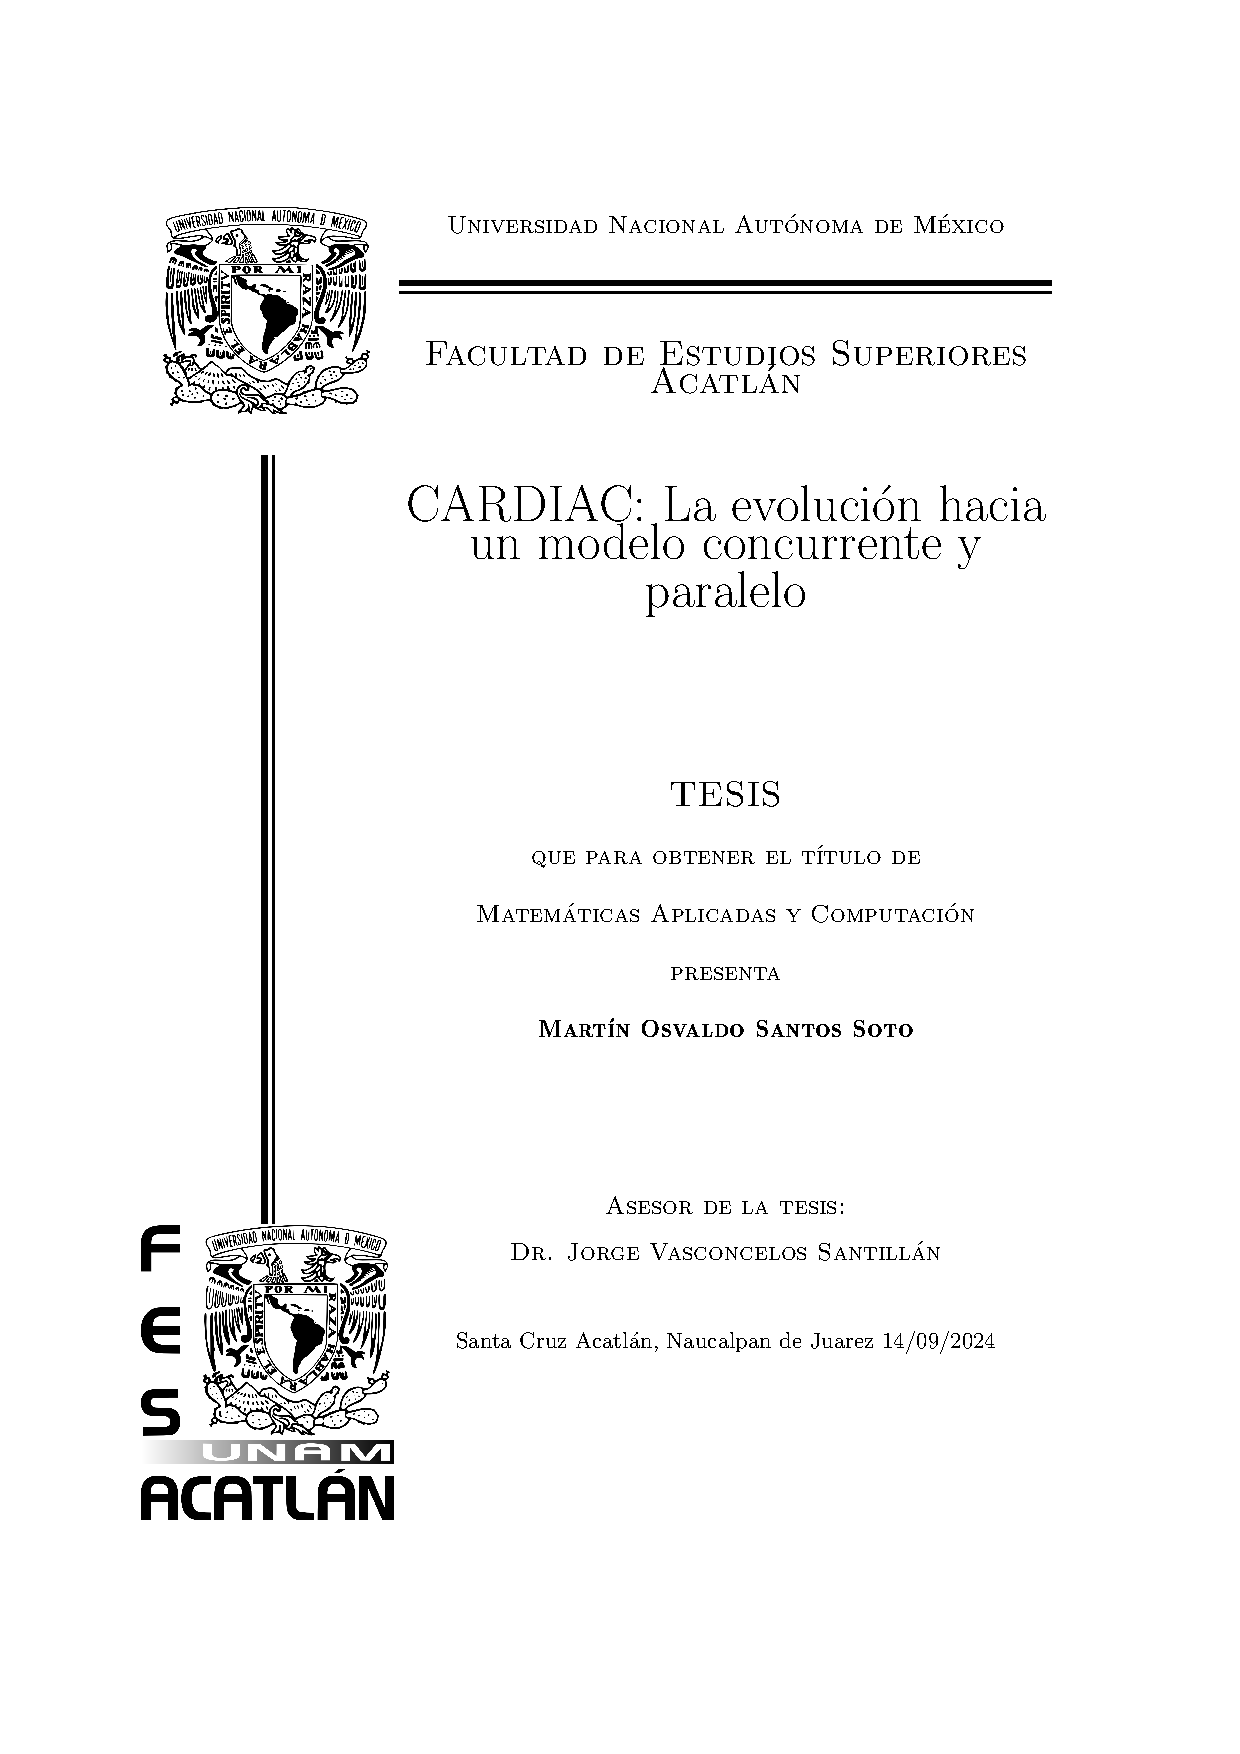
\includepdf{media/cover.pdf}

%---------------------------------
\chapter*{}
\begin{flushright}%
  \emph{A la facultad que me permitió crecer...}
  \thispagestyle{empty}
\end{flushright}

\chapter{Agradecimientos}
%\spacing{1.5}%\doublespacing

\chapter{Abstract}

\chapter{Introducción}

	Hoy en día tenemos multitud de aparatos electrónicos que pueden ser llamados computadoras; celulares, laptops, tabletas, relojes inteligentes, y un sin fin más. 
	Estos aparatos pueden ser llamados así siempre que sean  capaces de resolver operaciones aritméticas y lógicas de manera automática, al menos en la definición
	más aceptada que recoge el diccionario de Cambridge(dado que la palabra de origen es anglosajona en este contexto),
	por que sin analizamos más meticulosamente el termino ``computadora''  notaremos que el origen de la palabra es anterior a las computadoras
	tal cual las conocemos hoy día, por ejemplo las primeras nociones de ``computadoras''  eran referidas a mujeres de los años 1930 en estados unidos
	que trabajaban en la NASA y realizaban cálculos manuales, por ende podemos deducir que ese termino fue cambiando hasta ser lo que es hoy.
	Si analizamos la historia notaremos que el avance científico en cuanto a maquinas
	que pudieran automatizar tareas que realizaba la humanidad estaban centrados en las calculadoras, había que hacer los cálculos matemáticos menos
	complejos, ya sea con la invención de maquinas o bien con técnicas como los logaritmos y las tablas de multiplicar que se tenían
	para consultar más rápidamente operaciones complejas y repetitivas, pero con el tiempo el mismo desarrollo de estas maquinas dio paso a algo más,
	a una maquina de propósito general, programable y que ya no solo resolvía operaciones aritméticas, sino que hacía pruebas lógicas y podías
	adaptarla a problemas más particulares, así se fueron formando las ``computadoras''.
	
	%%https://www.smithsonianmag.com/science-nature/history-human-computers-180972202/
	
	Podemos ahondar en está relación de las calculadoras y las computadoras si regresamos al siglo 19, para ir un poco a los orígenes de la computación,
    más precisamente en el año 1830 el entusiasta Charles Babbage había desarrollado una maquina llamada ``Diferential Engine''
	que resolvía ecuaciones matemáticas, una calculadora potente si lo queremos ver desde otra perspectiva. Pero su empeño en los siguientes años 
	se centraría en el diseño y constricción
	de su ``Analytical Engine'', que aunque fue imposible de construir por la tecnología de la época, ya fue pensada como una computadora
	de propósito general, en el sentido que podía hacer cálculos y resolver operaciones lógicas además de que era una maquina que se podía programar,
	cumpliendo así todos los puntos básicos para poder ser considerada como una computadora, pero lamentablemente no pudo llegar a ver la luz de la mano
	de su creador.
	
	En esté sentido podemos ver que las computadoras, o más bien su creación ha llevado mucho tiempo para concretarse en lo que tenemos hoy, que es algo mucho
	más complejo que una calculadora, y aunque sabemos de la complejidad de estos aparatos cuando vemos alguno ¿ analizamos como es que funcionan por dentro? ¿ como podemos enviar mensajes de texto mientras escuchamos la canción del momento?
	usualmente la respuesta es ``No'', que no es necesariamente una respuesta mala, como personas en nuestro día a día no podemos detenernos a analizar cada artefacto que tengamos cerca o usemos, a pesar de que sería muy útil saberlo
	si funciona el aparato es todo lo que necesitamos saber, después de todo hay muchas situaciones o cosas más importantes
	a las cuales prestar atención. Sin embargo, para los profesionales del área de la computación o tecnología en general, así como a aquellos interesados
	por estás tecnologías son preguntas que no pueden faltar. Y es que incluso si tu trabajo es el desarrollo web o
	el diseño de gráficas(que parecieran disciplinas muy lejanas al funcionamiento de un ordenador) entender las razones por las cuales tu computadora o las computadoras para las cuales desarrollas programas pueden hacer cómputos
	en paralelo o tener la potencia que tienen es fundamental para poder optimizar tus desarrollos, que decir si tu trabajo es la parte del hardware, en ese
	caso debes estar totalmente involucrado con el funcionamiento interno de las computadoras.
	Más aún, considero que al igual que en toda disciplina la historia de la misma o de los artefactos que estudia está debe ser conocida por
	los interesados en la disciplina, pero sobretodo por los profesionales, dado que hay que entender como ha sido la evolución, lo que ha cambiado
	y aquello que a pesar de los años sigue vigente y la razón por la cuál sigue vigente.
	
	Pero entender la historia de la computación podría parecer tedioso o complicado, 
	por que a pesar de que la historia de las computadoras modernas es corta hablando del tiempo
	de la humanidad, es larga a nivel de la evolución que ha habido en los últimos 80 años, y esto es lo que puede parecer tedioso, sólo hay que ver las diferencias entre
	las computadoras actuales y aquellas que corrían con Windows 98, la diferencia ya es enorme. Ahora si vamos más  a las primeras computadoras personales
	que aún corrían unicamente con línea de comandos y con un paradigma de uso muy diferente al nuestro podemos notar que el cambio ha sido gigante, con todos estos
	cambios uno podría llegar a pensar que una computadora actual ya no tiene prácticamente nada que ver con los ``gigantes de hierro'' de los años 1950, 
	aunque en realidad no es tan simple y de hecho hay muchas similitudes entre estás computadoras. Es más a día de hoy la arquitectura, la estructura
	más general de una computadora actual es exactamente la misma que la de varias de las primeras computadoras, con mejoras en la potencia de
	procesamiento lógicamente, pero con una misma estructura y entender por que esa estructura se ha mantenido vigente hasta nuestros días nos
	llevará a entender lo importante que fue su creación. Analizando la historia de esa manera, estableciendo conexiones y conociendo que fue lo que continuo
	y que no ayuda a que esa gigantesca línea del tiempo de las computadoras adquiera otro tono, un tanto menos tedioso, que no se quede
	montón de fechas y que más bien sea una guía de cambios o sucesos que moldearon el mundo de la computación a lo que hoy conocemos.
	
	 
	Estás preguntas, este análisis se dio a largo de mi carrera universitaria, y 
	para resolverlo me encontré con algunos problemas, la barrera del idioma, dado
	que la lengua franca de la computación es en inglés muchos escritos están en ese idioma, y aunque hay muchos traducidos, otros más, en especial aquellos más 
	relacionados a partes antiguas de la computación no lo están. Otro,los 
	manuales
	o libros sumamente técnicos acerca del funcionamiento de los ordenadores, de como funciona el paralelismo, de las necesidades y utilidad del sistema operativo, que
	son realmente difíciles de leer para un estudiante que va empezando en la carrera. Este problema no es nuevo, ya se habían enfrentado a el no solo muchos
	estudiantes desde la aparición de la computación, sino también muchas instituciones y empresas que querían que más personas aprendieran a usar una computadora,
	que cabe mencionar que para esto es relevante el contexto histórico, dado que en los años 50 y 60 si querías usar una computadora tenías que entender muy bien el como funcionaba,
	no había una interfaz gráfica y un sistema operativo que hiciera todas las tareas secundarías por ti, tenías que entender como se movía por dentro la computadora para
	poder programar y resolver tus problemas. Es aquí, en este periodo histórico, más precisamente en los años 60, cuando varias compañías e instituciones
	educativas comienzan a lanzar ciertos modelos, manuales y kits para que los estudiantes aprendieran a usar computadoras tales como Little Man Computer lanzado por
	Madnick en los años 60, que básicamente era un kit de papel con un manual, una ``computadora de papel'' como se les ha llamado, en la cual tu como estudiante
	podías ver como eran las ejecuciones del código que habías escrito, y como eso se materializaba en una respuesta a tu problema inicial. Una de estás fue 
	``Little Man Computer(LMC)'' creada por Stuart Madnick y Jhon Donovan del MIT en los años 60, que con un reducido set de instrucciones permitía a los estudiantes probar la
	ejecución de programas como si estuvieran en una computadora real, otra de mucha relevancia fue su contemporánea CARDIAC(CARDboard Illustrative Aid to Computation) 
	desarrollada por Bell Labs de la mano de David W. Hagelbargery Saul Fingerman, que es
	muy similar a lo descrito sobre LMC, pero con su propio lenguaje y su propia arquitectura, que incluso llego a ser  más popular
	por el poder de Bell Labs en aquellos tiempos. Hubo otros desarrollos en años siguientes que tenían el mismo fin y es que en los años de 1960
	las computadoras eran ordenadores gigantes y conseguir tiempo para usarlos era realmente difícil, comprarlos directamente imposible para las personas
	comunes, entonces la solución que encontraron para que los estudiante pudieran practicar es la creación de estos kits con computadoras de papel, que los
	preparaban  para cuando pudieran usar una computadora ``real''.
	
	Eso quizá nos pueda parecer una simple clase de historia de la computación, pero no lo es, CARDIAC sigue siendo muy útil y de hecho
	funciona para explicar una buena parte del funcionamiento de a las computadoras, yo experimente el uso de CARDIAC en una clase de programación paralela y concurrente en la 
	cual esté modelo
	fue fundamental para entender los conceptos básicos de los que parte la computación. También hay que entender que con CARDIAC no te vas a volver un experto en 
	el funcionamiento de las computadoras,
	pero el punto es entender de una forma clara su estructura de modo que tengas las bases para entonces ser capaz de leer uno de esos manuales gigantes sobre sistemas
	operativos y arquitectura de computadoras con muchísimos conceptos técnicos, los cuales si no tienes cierto conocimiento de base pueden
	parecer muy complicados.
	
	Aún con todas estás ventajas de CARDIAC, las limitaciones son evidentes, fue construida en el año 1968, no es apta para la concurrencia ni el paralelismo, o 
	incluso un computo distribuido, por esa razón muchas personas que están en el mundo de la computación en los años posteriores han seguido haciendo
	modelos similares como MARIE(Machine Architecture that is Really Intuitive and Easy) o directamente evoluciones de ella como TIMBA(Terrible Imbecile Machine for Boring 
	Algorithms), algunos más técnicos que otros, y aunque la mayoría están en inglés hay varios proyectos en español. 
	Al adentrarme más en estos modelos me di cuenta que un buen modelo que explicará el funcionamiento de computadoras más avanzadas se volvían más técnicos, como el 
	desarrollo mexicano de \textit{8 bit a complete Design}, 
	que es un gran trabajo, pero que termina siendo bastante técnico y los demás que no son tan técnicos caen un poco en ser bastante similares a CARDIAC, lo cual no 
	es malo, e incluso tiene muchas ventajas que mejoran algunas lagunas de CARDIAC, pero hay otras más que no solucionan. Es en esté punto en el que decidí empezar este
	proyecto de investigación para explicar como funcionan las computadoras de una forma simple y didáctica para aquellos estudiantes que van empezando la carrera,
	tomando como base el  desarrollo de CARDIAC y llevándola unos pasos más allá en nivel de arquitectura para que sea capaz de explicar
	la computación concurrente y paralela, así como entender la necesidad de un sistema operativo en maquinas más complejas sin dejar de lado la simplicidad que la 
	caracteriza.
	Con un enfoque particular que lleve al lector a ver las necesidades de hardware y software que hacen evolucionar a CARDIAC,
	de forma que se entienda las necesidades que llevaron a la evolución de las computadoras en varios ámbitos fundamentales, y en ese mismo sentido situarse en la línea
	temporal en que surgieron esos cambios para entender su contexto histórico y como lo mencione antes, entender por que hay características  que siguen vigentes
	70 años después en los ordenadores y otras no.
	
	
	Más allá del recorrido en la construcción y diseño de modelos ``evolucionados'' de CARDIAC para computación paralela y concurrente el texto se verá acompañado,
	tal como la clásica CARDIAC distribuida por Bell Labs, con un ``kit'' que incluye un programa que contendrá tres maquinas virtuales para cada
	modelo de CARDIAC, con la diferencia de que estas maquinas virtuales ya no serán en papel, sino interfaces gráficas para uso en computadoras de escritorio.



\tableofcontents
\listoffigures

\mainmatter

\chapter{Orígenes de la computación} %


\section{Inicios de la computación}
	\subsection{Primeros autómatas}
	% Breve historia de como se fue desarrollando la computación desde los inicios hasta llegar a automatas(1950)
	\subsection{Primeras computadoras}
	%1950-1970
	\subsection{Nacimiento de CARDIAC}
	%El como nace el modelo para dar claridad a los trabajadores de ATT
	\subsection{Evolución hasta la actualidad}
   
\section{Arquitecturas de computadoras}   
   
\subsection{Modelo concurrente}

\subsection{Modelo paralelo}


\chapter{Metodología}  %
	\section{Necesidad de operaciones concurrentes}
	
	 \section{Evolución hacia el paralelismo}

\chapter{Resultados}  %


\chapter{Conclusiones}

%\bibliographystyle{humannat}
%\bibliography{references}

%\backmatter%@sglvgdor


\end{document}

